\documentclass[main.tex]{subfiles}
\newcommand\numberthis{\addtocounter{equation}{1}\tag{\theequation}}

\newtheorem{theorem}{Theorem}[section] %Delete when merging subfiles
\newtheorem{corollary}{Corollary}[theorem]
\newtheorem{definition}{Definition}[section]

\allowdisplaybreaks

\begin{document}
\section{PAC-Learning and VC-Dimension}
In this section we will have a look to some statistical learning method.
Previously we focused our attention on estimating the generalization error of a given model in order to measure the true performance. The training error usually is not a good indicator of how a model is behaving, but is way easier to estimate than other error terms. So we would like to extract as many information as possible from training error. Also there are cases where the training error is somewhat a good estimation of the performance. For example when we have a good number of samples relative to our hypothesis space we are less prone to overfitting. A question arises naturally. Can we estimate how many samples are necessary given an hypothesis space? We can answer this question in a theoretical way. Please remind that from a practical point of view it is rarely used.
\subsection{PAC-Learning}
To introduce the ingredients of the theoretical setting we use a character recognition task. Given an array of n bits encoding a binary-valued image we have
\begin{itemize}
    \item X \textbf{Instances set}. In the character recognition problem, the instance space is $X=\{0,1\}^{n}$. The set of all possible input binary images.
    \item H \textbf{Hypothesis space}. The space where lies all possible combination of parameters.
    \item C \textbf{Set of target concept}. A concept is a subset $c\subset X$. One concept is the set of all patterns of bits in  $X=\{0,1\}^{n}$ that encode a picture of the letter "P".
    \item $\mathcal{P}$ \textbf{Probability distribution over X}. Training instances are generated by a fixed, unknown probability distribution over X
\end{itemize}
The learner observes a sequence $\mathcal{D}$ of training example $<x,c(x)>$ for some target concept $c \in C$ and $x$ is drawn from $\mathcal{P}$. The learner must output a hypothesis h estimating c. h is evaluated by its performance on subsequent instances drawn according to $\mathcal{P}$
\begin{equation*}
    L_{true} = P_{x \in \mathcal{P}}(c(x) \neq h(x))
\end{equation*}
Our objective is to bound $L_{true}$ given $L_{train}$.
Now we introduce the so called \textbf{version space} $VS_{H,\mathcal{D}}$. It is a subset of H where the training error $L_{train}$ is zero. So the hypothesis h are always correct on training instances. For now, we assume that VS is non-empty. Making some consideration we can bound $L_{train}$ inside VS.
\begin{theorem}[$L_{train}$ bound in VS]
    If the hypothesis space H is finite and $\mathcal{D}$ is a sequence of $N \geq 1$ independent random examples of some target concept c, then for any $0 \leq \epsilon \leq 1$, the probability that $VS_{H,\mathcal{D}}$ contains a hypothesis error greater then $\epsilon$ is less than $|H|e^{-\epsilon N}$:
    \begin{equation*}
        P(\exists h \in H: L_{train}(h)=0 \land L_{true}(h) \geq \epsilon) \leq |H|e^{-\epsilon N}
    \end{equation*}
\end{theorem}

\newpage
\begin{proof}
    $$P((L_{train}(h_1)=0 \land L_{train}(h_1) \geq \epsilon) \lor \dots \lor (L_{train}(h_{|H|})=0 \land L_{train}(h_{|H|}) \geq \epsilon))$$
    \begin{align*}
         & \leq \sum_{h \in H} P(L_{train}(h)=0 \land L_{train}(h) \geq \epsilon) & \text{Union bound}                                               \\
         & \leq \sum_{h \in H} P(L_{train}(h)=0 | L_{train}(h) \geq \epsilon)     & \text{Bound using Bayes’ rule}                                   \\
         & \leq \sum_{h \in H_{bad}} (1-\epsilon)^N                               & \text{Bound on individual }h_is                                  \\
         & \leq |H|(1-\epsilon)^N                                                 & |H|_{bad}\leq|H|                                                 \\
         & \leq |H|e^{-\epsilon N}                                                & (1-\epsilon \leq e^{-\epsilon},for \quad 0 \leq \epsilon \leq 1)
    \end{align*}
\end{proof}
We can notice that the dimension of the hypothesis space influences negatively the bound, in fact a larger searching space will give us less guarantees on the value of $L_{true}$. On the other hand, having more samples is always better, in fact $e^{-\epsilon N}$ is monotonically decreasing with N. Larger $\epsilon$ will lead to smaller bound because we are less demanding on the similarity between $L_{true}$ and $L_{train}$.
Now we can bound the probability of $P(\exists h \in H: L_{train}(h)=0 \land L_{true}(h) \geq \epsilon) \leq |H|e^{-\epsilon N}$. We can set a parameter $\delta$
\begin{equation*}
    |H|e^{-\epsilon N} \leq \delta
\end{equation*}
After choosing $\delta$ we can calculate N or $\epsilon$.\\
Given $\epsilon$ and $\delta$
\begin{equation}
    N \geq \frac{1}{\epsilon} \bigg( ln(|H|) + ln \bigg( \frac{1}{\delta} \bigg) \bigg)
\end{equation}
Given N and $\delta$
\begin{equation}
    \epsilon \geq \frac{1}{N} \bigg( ln(|H|) + ln \bigg( \frac{1}{\delta} \bigg) \bigg)
\end{equation}
\paragraph{Note} $|H|$ can be very large. If we take as an example a binary decision problem with M binary inputs(features), the size of H will be $2^{2^M}$. So N will have a exponential relationship with M. This is related to the curse of dimensionality.
\paragraph{Example} Suppose H contains conjunctions of constraints on up to M boolean attributes (i.e., M literals). In this case $|H|=3^M$. How many examples are sufficient to ensure with probability at least $(1-\delta)$ that every h in $VS_{H,\mathcal{D}}$ satisfies $L_{true}(h) \leq \epsilon$?
\begin{align*}
    N & \geq \frac{1}{\epsilon} \bigg( Mln(3) + ln \bigg( \frac{1}{\delta} \bigg) \bigg)
\end{align*}
\newline
Now we are ready to define formally what PAC\footnotemark is. Consider a class C of possible target concepts defined over a set of instances X of length n, and a learner L using hypothesis space H. \footnotetext{Probably Approximately Correct learning. Probably refers to $\delta$ and it is the confidence. Approximately refers to $\epsilon$ and it is the accuracy}
\begin{definition}
    C is \textbf{PAC-learnable} if there exists an algorithm L such that for every $f \in C$, for any distribution $\mathcal{P}$, for any $\epsilon$ such that $0 \leq \epsilon < \frac{1}{2}$, and $\delta$ such that $0 \leq \delta < \frac{1}{2}$, then algorithm L, with probability at least $(1-\delta)$, outputs a concept h such that $L_{true}(h) \leq \epsilon$ using a number of samples that is polynomial of $\frac{1}{\epsilon}$ and $\frac{1}{\delta}$
\end{definition}
\begin{definition}
    C is \textbf{efficiently PAC-learnable} by L using H $\iff$ $\forall c \in C$, distributions $\mathcal{P}$ over X, $\epsilon$ such that $0 \leq \epsilon < \frac{1}{2}$, and $\delta$ such that $0 \leq \delta < \frac{1}{2}$, algorithm L, with probability at least $(1-\delta)$, outputs a concept h such that $L_{true}(h \leq \epsilon)$, in time that is polynomial in $\frac{1}{\epsilon}$, $\frac{1}{\delta}$, M and size(c)\footnotemark
\end{definition} \footnotetext{size(c): Number of bit necessary to express c. It comes from information theory}

Now we need to generalize to problems where the VS is empty, because usually the train error is not equal to zero(agnostic learning). We can simply bound the difference between $L_{train}$ and $L_{true}$ in H.
\begin{equation*}
    L_{true}(h) \leq L_{train} + \epsilon
\end{equation*}
From now on we will consider only binary classification problems for simplicity. As we did before, we need to find an upper bound for the probability of having a "bad event", which in this case consists in having a gap between $L_{train}$ and $L_{true}$ bigger than $\epsilon$. To achieve this we use the \textbf{Hoeffding bound}, which states
\begin{definition}
    For N i.i.d. coin flips $X_1, \dots, X_N$, where $X_i \in \{0,1\}$ and $0 < \epsilon < 1$, we define the empirical mean $\Bar{X}=\frac{1}{N}\sum_{i=1}^N X_i$, obtaining the following bound
    \begin{equation*}
        P(E[\Bar{X}]-\Bar{X} > \epsilon) \leq e^{-2N\epsilon^2}
    \end{equation*}
\end{definition}
\begin{theorem}
    Given an hypothesis space H, a dataset $\mathcal{D}$ with N i.i.d. samples, $0< \epsilon <1$: for any learned hypothesis h:
    \begin{equation*}
        P(\exists h \in H | L_{true}(h)-L_{train}(h) > \epsilon) \leq |H|e^{-2N \epsilon^2}
    \end{equation*}
\end{theorem}
This is very similar to what we have found in the non-empty case. Like we did before, we can calculate the number of example needed given $\epsilon$ and $\delta$
\begin{equation*}
    N \geq \frac{1}{2 \epsilon^2} \bigg( ln(|H|) + ln\bigg( \frac{1}{\delta} \bigg) \bigg)
\end{equation*}
Or $\epsilon$ given N and $\delta$.
\begin{equation*}
    \epsilon \geq \sqrt{\frac{ln(|H|) + ln( \frac{1}{\delta} )}{2N}}
\end{equation*}
Now we can rewrite the gap between $L_{train}$ and $L_{true}$ as
\begin{equation}
    L_{true}(h) \leq \underbrace{L_{train}(h)}_{Bias} + \underbrace{\sqrt{\frac{ln(|H|) + ln( \frac{1}{\delta} )}{2N}}}_{Variance}
\end{equation}
Once more, we can see how $|H|$ influences the loss function. For large $|H|$ we assume a low bias because it's more probable to find a good h and a high variance. For small $|H|$ we have high bias because we have a low probability of including a good h and low variance. In practice what we are saying is that we have to justify a large H with a lot of data. If we do so the training error will be a good estimation of the overall performance(test/true error).

\subsection{VC Dimension}
So far we have considered only finite hypothesis space. If we use the bound that we have just found in an infinite\footnotemark H, we would have infinite variance. This is not the case, for infinite H the previous bound is too pessimistic. So we need to find a new one\footnotetext{Infinite hypothesis spaces are very common. For example linear regression or classification have infinite hypothesis spaces}. In the finite H case we encoded the complexity of H in the number of possible hypothesis. In the infinite case we can't do this, so we need to find a new metric to measure the complexity of H. We will use the \textbf{VC dimension}. To lay the ground for our theoretical discussion, we need to introduce two definitions,
\begin{definition}[Dichotomy]
    A dichotomy of a set S is a partition of S into two disjoint subsets
\end{definition}
\begin{definition}[Shattering]
    A set of instances S is shattered by hypothesis space H if and only if for
    every dichotomy of S there exists some hypothesis in H consistent with this
    dichotomy
\end{definition}
In practice shattering means that if we split our instances set in two not overlapping subset, H shatters S if and only if for every dichotomy we can find an hypothesis which classify correctly every instances. As a reminder we are still considering only binary classification problems.
\paragraph{Example} We consider an instances set with three example\footnotemark and an hypothesis space representing a linear classifier. In this case a dichotomy is a specific assignment of class (+) or class (-) to every point. We can have two cases, one where the examples are not aligned and one where they are. H shatters any of the two instances set? Yes, only (a) because we can always find a line that divides every possible dichotomy. In the specific dichotomy shown for (b), we can't find a linear classifier(line), that classifies correctly the three points, so H doesn't shatter (b). \footnotetext{This is still infinite because every instance can have a different "position" in the instances set}
\begin{center}
    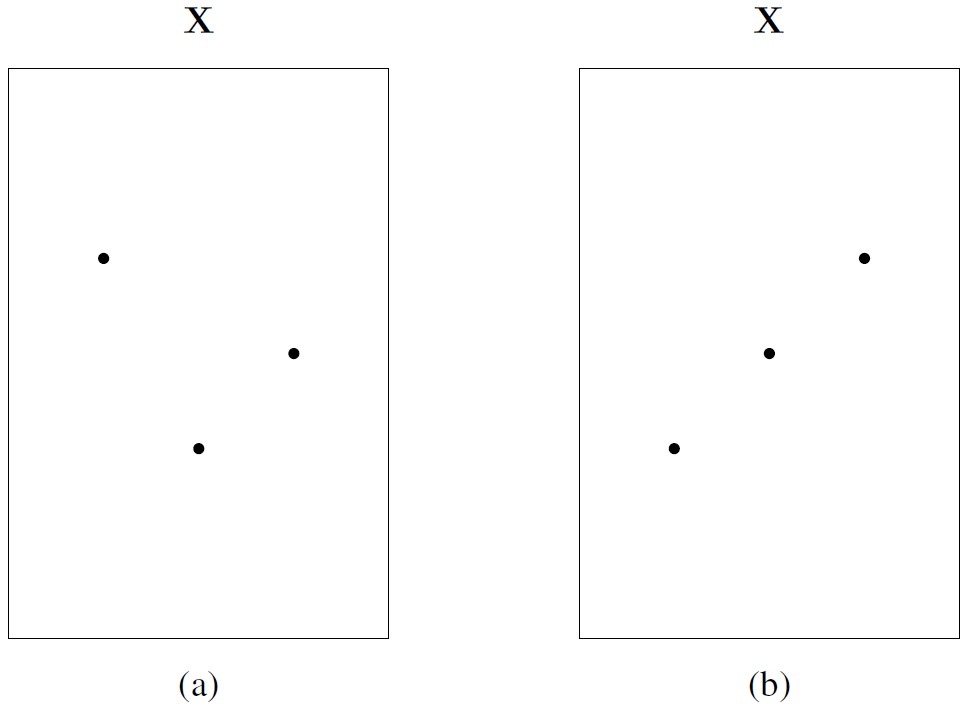
\includegraphics[height=80mm]{img/VC_example.PNG}
\end{center}
\begin{center}
    \begin{tabular}{ccc}
        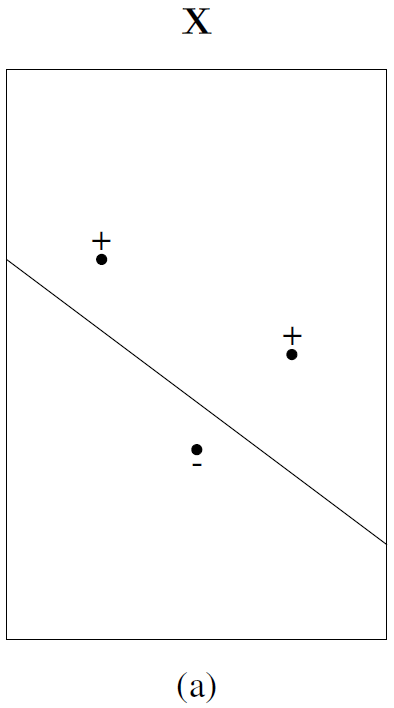
\includegraphics[height=80mm]{img/VC_example2.PNG} & 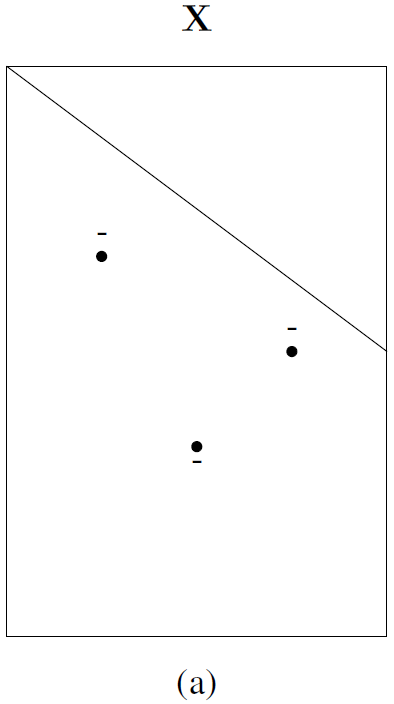
\includegraphics[height=80mm]{img/VC_example3.PNG} &
        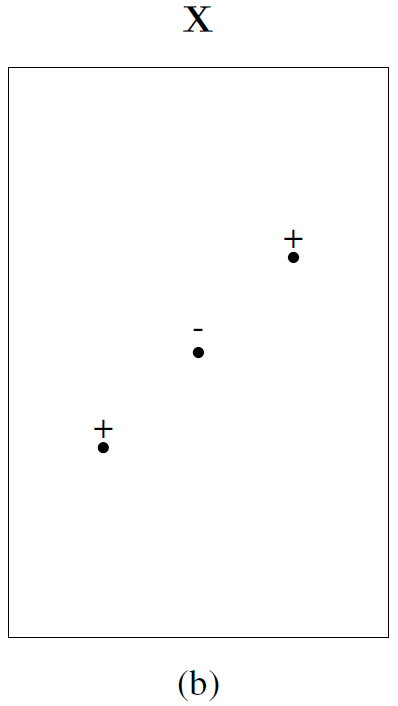
\includegraphics[height=80mm]{img/VC_example4.PNG}
    \end{tabular}
\end{center}
Note that for four instances, H won't shutter S.\footnotemark \footnotetext{This is the XOR problem. It's not linearly separable}
Now we can define what is the VC dimension
\begin{definition}[VC dimension]
    The Vapnik-Chervonenkis dimension, $VC(H)$, of hypothesis space H
    defined over instance space X, is the size of the largest finite subset of X shattered by H. If arbitrarily large finite sets of X can be shattered by H, then $VC(H) \equiv \infty$
\end{definition}
In our previous example, the VC dimension of linear classifiers in two dimension is three. In fact, we can have a configuration of three instances whereby every dichotomy is perfectly separable. This doesn't hold for four instances.
\paragraph{Example} Few examples of VC dimensions,
\begin{itemize}
    \item Linear classifier: $VC(H) = M+1$, for $M$ features plus the constant term.
    \item Neural networks: $VC(H) = \#parameters$
    \item 1-Nearest Neighbor: $VC(H) = \infty$
    \item SVM with Gaussian Kernel: $VC(H) = \infty$. We will see SVM in future chapters.
\end{itemize}
Now we can find a new bound for the error between $L_{train}$ and $L_{true}$, and so we can find how many randomly drawn examples suffice to guarantee an error of at most $\epsilon$ with probability at least $(1-\delta)$
\begin{equation}
    N \geq \frac{1}{\epsilon} \bigg( 4log_2 \bigg( \frac{2}{\delta} \bigg) + 8VC(H) log_2 \bigg( \frac{13}{\epsilon} \bigg) \bigg)
\end{equation}
Equally we can express this as an upper bound for $L_{true}$
\begin{equation}
    L_{true}(h) \leq L_{train}(h) + \sqrt{\frac{VC(H)(ln(\frac{2N}{VC(H)})+1)+ln(\frac{4}{\delta})}{N}}
\end{equation}

\paragraph{Properties}
\begin{theorem}
    The VC dimension of a hypothesis space $|H| < \infty$ is bounded from above
    \begin{equation*}
        VC(H) \leq log_2(|H|)
    \end{equation*}
\end{theorem}
\begin{proof}
    If $VC(H)=d$ then there exists at least $2^d$ functions(combination) in H, since there are at least $2^d$ possible labelings
    \begin{align*}
        |H|   & \geq 2^d        \\
        |H|   & \geq 2^{VC(H)}  \\
        VC(H) & \leq log_2(|H|)
    \end{align*}
\end{proof}
\begin{theorem}
    Concept class C with $VC(C) = 1$ is not PAC-learnable.
\end{theorem}

\newpage

\end{document}
